% ==============================================================
%  Chapter 4 -- Experimental Study
% ==============================================================

\chapter{Experimental Study}
\label{ch:experiments}

This chapter puts the pipeline of Chapter~\ref{ch:implementation} to
the test on two real influence diagrams of clinical origin. The
\emph{bypass} diagram, already introduced in
Section~\ref{sec:bypass-example} as the running example of the
implementation, plays the role of a small sanity-check benchmark
where the parameter recovery can be tracked node by node. The
\emph{NHLv1} diagram, presented in the next section, is one order of
magnitude larger and constitutes the main benchmark of the empirical
study.

% ==============================================================
\section{Benchmark networks}
\label{sec:benchmarks}
% ==============================================================

\subsection{NHLv1: management of non-Hodgkin lymphoma}
\label{sec:nhlv1}

The \emph{NHLv1} influence diagram models the clinical management of
gastric non-Hodgkin lymphoma. Its qualitative structure is shown in
Figure~\ref{fig:nhlv1-id}. It comprises sixteen chance nodes
covering disease, treatment-side-effect and outcome variables, three
decision nodes (\textsf{Surgery}, \textsf{Helicobacter treatment} and
\textsf{CT-RT schedule}) and a single utility node. Because of its
size and connectivity, the parameter vector
$\boldsymbol{\Theta}$ associated with the diagram is of the order of
several thousand entries, which makes the elicitation bottleneck
discussed in Chapter~\ref{ch:introduction} fully tangible and the
EDA-based recovery the only practical route to populating the
network.

\begin{figure}[H]
    \centering
    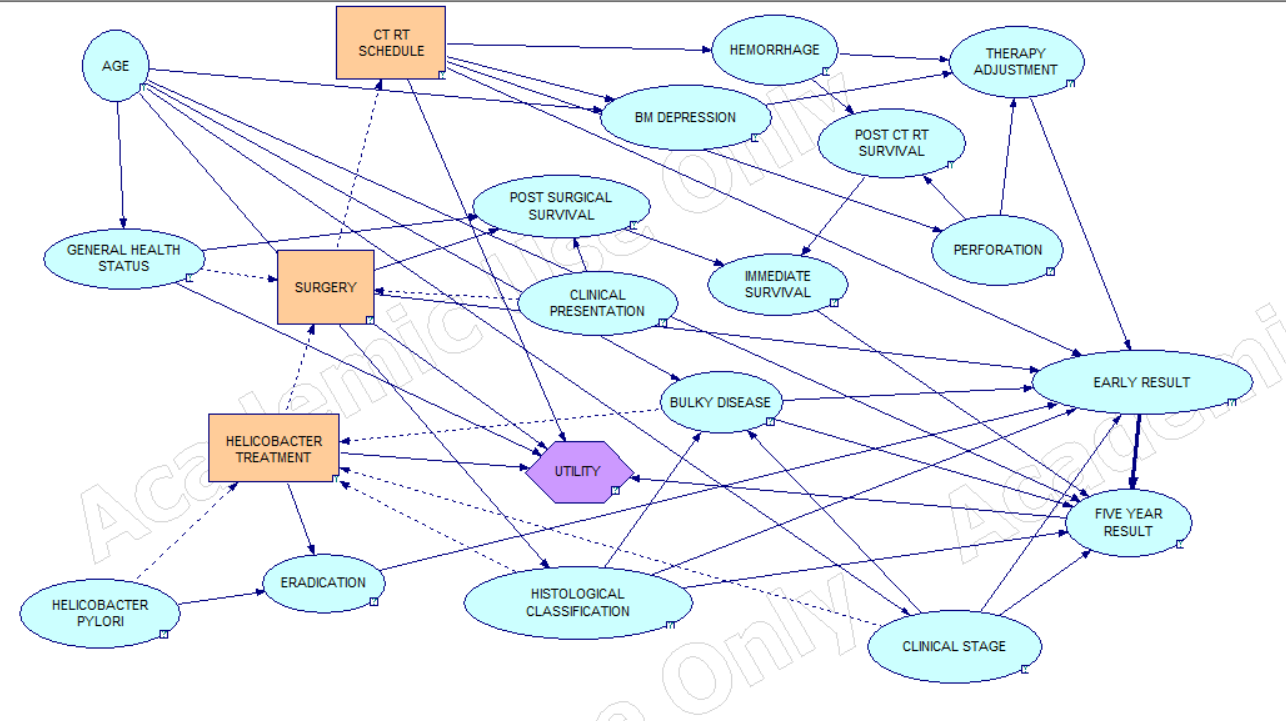
\includegraphics[width=0.95\linewidth]{figures/nhlv1.png}
    \caption{Influence diagram of the \emph{NHLv1} model for the
    management of gastric non-Hodgkin lymphoma. Chance nodes are
    ellipses, decision nodes rectangles and the utility node a
    hexagon. Dashed arcs are informational, solid arcs are
    probabilistic or functional. The model is the main benchmark of
    this work.}
    \label{fig:nhlv1-id}
\end{figure}

\subsection{Bypass: management of coronary heart disease}
\label{sec:bypass-bench}

The \emph{bypass} diagram was already presented in
Section~\ref{sec:bypass-example} as the illustrative model used to
explain the implementation. It is reused here as a small, controlled
benchmark on which the parameter vector is small enough for a finer
ablation study of the encoding, the decoding, the loss and the EDA
variant.

% ==============================================================
\section{Experimental protocol}
\label{sec:protocol}
% ==============================================================

% TODO: describe the hyperparameter sweep, the metrics
% (rule accuracy, MSE w.r.t. true CPTs, MSE w.r.t. true utility,
% utility deviation, normalised entropy, training/validation split,
% number of repetitions, random seeds, hardware).

\bigskip
\textbf{[To be completed.]}

% ==============================================================
\section{Results}
\label{sec:results}
% ==============================================================

% TODO: present the results grouped by axis of the sweep:
%  - EDA variant (UMDA vs EMNA vs EGNA vs KEDA)
%  - loss function (binary / regret / margin / softmax / entropy)
%  - temperatures (chance / utility)
%  - selection ratio alpha and population size
%  - symmetric vs non-symmetric sampling
%  - min_max_ut on/off
%  - mode (both / chance_only / utility_only)
%  - effect of rule-base size

\bigskip
\textbf{[To be completed.]}

% ==============================================================
\section{Discussion}
\label{sec:discussion}
% ==============================================================

% TODO: summarise the empirical findings, link them back to the
% theoretical analysis of Chapter 2 (non-convexity, degeneracy),
% and highlight the limits.

\bigskip
\textbf{[To be completed.]}
